\documentclass[11pt,a4paper,oneside]{article}
\usepackage[utf8]{inputenc}
\usepackage{amsmath}
\usepackage{amsfonts}
\usepackage{amssymb}
\usepackage{graphicx}
\usepackage{color}
\usepackage {tikz}
\usetikzlibrary {er}
\usepackage[left=2.00cm, right=2.00cm, top=1.00cm]{geometry}
\graphicspath{{./}}
\input glyphtounicode


\begin{document}
	\title{DS 256 - Scalable Systems for Data Science \\ Assignment 0}
	\author{Shriram R. \\ M Tech (CDS) \\ 06-02-01-10-51-18-1-15763}
	\maketitle
	
	\section{Introduction}
	Analytics of Twitter data has been performed using Apache Spark through its Java interface. The experimental setup, results, plots and analysis are described in detail in the following sections.
     
    \section{Experimental Setup}
    
    \subsection{Hardware}
    Experiments were performed on a commodity cluster having 24 compute nodes. Each node has a 8-core AMD Opteron 3380 processor clocked at 2.6Ghz along with 32GB RAM and 2TB HDD and runs Ubuntu 16.04 LTS (64 bit) with Linux 4.4.0-139-generic. The nodes are connected through a Gigabit Ethernet switch.
    
    \subsection{HDFS and Spark}
    The HDFS environment has a capacity of 30.93TB with block size 128MB, replication factor of 2 and heartbeat delay of 3s. The global configuration of Spark for all experiments is 4 executors (containers) each having 4 cores and 8GB of memory. The Driver memory was set to 512MB. Apache YARN was used to coordinate the job execution. Experiment specific detail if any is provided below.
    
    \subsection{Dataset}
    The dataset used is a collection of tweets from Twitter between 17th Oct - 16th Dec 2016. The total dataset size is about 955GB and is stored in HDFS by partitioning the dataset into 3984 files of comparable size. Each tweet is described in Twitter Tweet JSON format and is of size approximately 5-10KB . The structure of JSON is described in [1].
  
    \section{Histogram}
    The pseudocode for the histogram of hashtags per tweet is given below,
    
    \begin{verbatim} 
          // Load text file into RDD
       1. JavaRDD twitterData = textFile(inputFile)
          // Parse JSON and get the hash count along with User ID
       2. JavaPairRDD hashCount = twitterData.flatMapToPair(getHashCount()) 
          // Get the average hashtag per tweet for each user
       3. JavaRDD avgPerUser = hashCount.reduceByKey(x, y -> x+y).map(sum/count)
          // Get the bucket values and frequencies for the given bucket count
       4. histogram = avgPerUser.histogram(bucketCount)
       5. Write histogram to HDFS     
    \end{verbatim}    
    The job was executed for the full dataset using the global configuration. The job took about 2.9 hours to complete. The job initially sustained failed stages which took about 4.5 hours. This occurred due to failure in metadata fetch. The job generated about 17.9GB of Shuffle data. Bucket count was chosen arbitrarily as 20 and the result is plotted below,
    
    \begin{center}
    	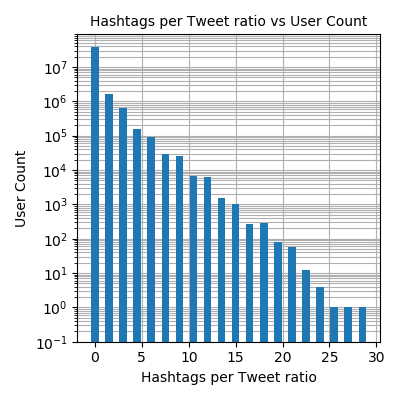
\includegraphics[scale=0.6]{1.png}		
    \end{center}

	It can be observed that the user count decreases as the Hashtag per tweet ratio increases. About 93.5\% of the users fall in the first bucket. The maximum Hashtag per tweet ratio in the given dataset is about 28.5 and the average value is about 0.16.
	
	\section{Co-occurring Hashtags}
	The pseudocode for finding the top 100 frequently co-occurring hashtags is given below,
	
	\begin{verbatim}
	       // Load text file into RDD
	    1. JavaRDD twitterData = textFile(inputFile)
	       // Parse JSON and get the hash tag pairs available in each tweet
	    2. JavaPairRDD hashTags = twitterData.flatMapToPair(getHashTags()) 
	       // Get the count for each distinct hash tag pair, sort descending by value
	    3. JavaRDD hashCount = hashTags.reduceByKey(x, y -> x+y).mapToPair(swap key-value)
	                                                            .sortByKey(false)
	       // Get top 100 frequent hash tag pairs
	    4. pairs = hashCount.take(100)
	    5. Write histogram to HDFS 
	\end{verbatim}
	
	The job was executed for the full dataset using the global configuration. The job took about 2.8 hours to complete and generated 9.4GB of Shuffle data. The list of top 100 pairs of Hashtags is available in Appendix A. The frequency of occurrence od these pairs is plotted below, 
	
	 \begin{center}
		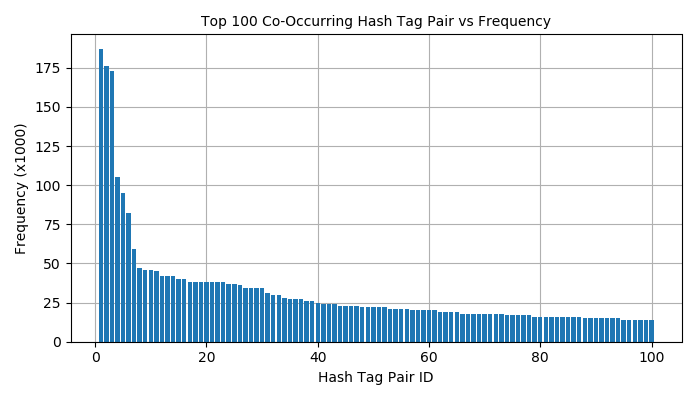
\includegraphics[scale=0.5]{2.png}		
	\end{center}

    The Hash Tag Pair IDs are alloted in the decreasing order of frequency. It can be observed that the frequency drops exponentially along the x-axis. The most frequent pair of Hash Tags was present in about 187,000 tweets. The Hash tags were from different languages.
    
    \section{Temporal Interaction Graph}
    
    The pseudocode for getting the temporal interaction graph is given below,
    
    \begin{verbatim} 
    // Load text file into RDD
    1. JavaRDD twitterData = textFile(inputFile)
    // Parse JSON and get the hash count along with User ID
    2. JavaPairRDD hashCount = twitterData.flatMapToPair(getHashCount()) 
    // Get the average hashtag per tweet for each user
    3. JavaRDD avgPerUser = hashCount.reduceByKey(x, y -> x+y).map(sum/count)
    // Get the bucket values and frequencies for the given bucket count
    4. histogram = avgPerUser.histogram(bucketCount)
    5. Write histogram to HDFS     
    \end{verbatim}
    
    The job was executed only on 1\% of the dataset. The job took a total of 9.1 minutes to complete and generated about 180MB of Shuffle data. Execution on larger dataset sizes resulted in job failures due to insufficient memory and/or workers getting disconnected and in some cases few tasks that were running indefinitely.   
    
    \section{References}
    \begin{list}{}{}
    	%\item 1. https://en.cppreference.com/
    	\item 2. DS 221 Course lecture notes
    	%\item 3. https://www.geeksforgeeks.org/
    	%\item 4. /home/shriramr/ds221/part\_3/code/test
    	%\item 5. /home/shriramr/ds221/part\_3/data/
    \end{list}

    \section{Appendix - A}
    
     \begin{center}
	    \begin{tabular}{|c|c|}
	    	\hline 
	    	\textbf{Hash Tag Pair ID} & \textbf{Hash Tag Pair} \\
	    	\hline
	    	1 & gameinsight,androidgames \\ 
	    	\hline
	    	2 & androidgames,android \\ 
	    	\hline
	    	3 & gameinsight,android \\ 
	    	\hline
	    	4 & ?????????,????????? \\ 
	    	\hline
	    	5 & ?????,BTS \\ 
	    	\hline
	    	6 & ???,GOT7 \\ 
	    	\hline
	    	7 & ?????,????? \\ 
	    	\hline
	    	8 & ??,JIMIN \\ 
	    	\hline
	    	9 & ????,TWICE \\ 
	    	\hline
	    	10 & ??,????? \\ 
	    	\hline
	    	11 & ?????,????? \\ 
	    	\hline
	    	12 & ???????,??????? \\ 
	    	\hline
	    	13 & ???????,????????? \\ 
	    	\hline
	    	14 & ?????????,??????? \\ 
	    	\hline
	    	15 & np,SoundCloud \\ 
	    	\hline
	    	16 & ??,? \\ 
	    	\hline
	    	17 & ??????,??????? \\ 
	    	\hline
	    	18 & ???????,?????? \\ 
	    	\hline
	    	19 & ????????????,?????? \\ 
	    	\hline
	    	20 & ????????????,??????? \\ 
	    	\hline
	    	21 & ???????,???????????? \\ 
	    	\hline
	    	22 & ?????????,?????? \\ 
	    	\hline
	    	23 & ?????????,???????????? \\ 
	    	\hline
	    	24 & ??????,???? \\ 
	    	\hline
	    	25 & job,Hiring \\ 
	    	\hline
	    	
	    	26 & ?,Hadith \\ 
	    	\hline
	    	27 & ??,????? \\ 
	    	\hline
	    	28 & ?,????? \\ 
	    	\hline
	    	29 & ??,????? \\ 
	    	\hline
	    	30 & ?????,????? \\ 
	    	\hline
	    	31 & ?????,MONSTA\_X \\ 
	    	\hline
	    	32 & ??,SUGA \\ 
	    	\hline
	    	33 & ?????,JIMIN \\ 
	    	\hline
	    	34 & ??,????? \\ 
	    	\hline
	    	35 & ?,???\_????? \\ 
	    	\hline
	    	36 & MTVStarsFifthHarmony,AP40FifthHarmony \\ 
	    	\hline
	    	37 & ????,GOT7 \\ 
	    	\hline
	    	38 & ???,SEVENTEEN \\ 
	    	\hline
	    	39 & MTVStars5SOS,AP405SOS \\ 
	    	\hline
	    	40 & ?????,SUGA \\ 
	    	\hline
	    	41 & GOT7,BamBam \\ 
	    	\hline
	    	42 & ??,V \\ 
	    	\hline
	    	43 & ??,VIXX \\ 
	    	\hline
	    	44 & Hiring,CareerArc \\ 
	    	\hline
	    	45 & ??,GOT7 \\ 
	    	\hline
	    	46 & ?????,????? \\ 
	    	\hline
	    	47 & EMABiggestFansBeyonce,ARIASBEYONCE \\ 
	    	\hline
	    	48 & Necklace,Jewelry \\ 
	    	\hline
	    	49 & ?????,V \\ 
	    	\hline
	    	50 & ??,JUNGKOOK \\ 
	    	\hline
	    	51 & JIMIN,BTS \\ 
	    	\hline
	    	52 & V,BTS \\ 
	    	\hline
	    	53 & ?,V \\ 
	    	\hline
	    	54 & KCAArgentina,5SOS \\ 
	    	\hline
	    	55 & job,CareerArc \\ 
	    	\hline
	    	56 & JB,GOT7 \\ 
	    	\hline
	    	57 & ?????,????? \\ 
	    	\hline
	    	58 & ?,BTS \\ 
	    	\hline
	    	59 & ??,GOT7 \\ 
	    	\hline
	    	60 & ?????,BTS \\ 
	    	\hline
	    	61 & ??,BTS \\ 
	    	\hline
	    	62 & ??,BTS \\ 
	    	\hline
	    	63 & ??,??? \\ 
	    	\hline
	    	64 & ??,BAEKHYUN \\ 
	    	\hline
	    	65 & ??,BamBam \\ 
	    	\hline
	    	66 & ??,BTS \\ 
	    	\hline
	    	67 & ???????????,????????? \\ 
	    	\hline
	    	68 & ?????,JUNGKOOK \\ 
	    	\hline
	    	69 & ??????,????? \\ 
	    	\hline
	    	70 & Mark,GOT7 \\ 
	    	\hline
	    	71 & ????????,ksa \\ 
	    	\hline
	    	72 & ipadgames,gameinsight \\ 
	    	\hline
	    	73 & ipadgames,ipad \\ 
	    	\hline
	    	74 & ??,??? \\ 
	    	\hline
	    	75 & ipad,gameinsight \\ 
	    	\hline
	    	76 & EMABiggestFansLadyGaga,EMABiggestFansArianaGrande \\ 
	    	\hline
	    	77 & ????????,saudi \\
	    	\hline
	    	78 & ??,Mark \\ 
	    	\hline
	    	79 & ???????,????????? \\ 
	    	\hline
	    	80 & ????,??? \\ 
	    	\hline
	    	81 & ?????,GUILTY \\ 
	    	\hline
	    	82 & Jobs,Job \\ 
	    	\hline
	    	83 & ?????,?????? \\ 
	    	\hline
	    	84 & saudi,ksa \\ 
	    	\hline
	    	85 & ??,GOT7 \\ 
	    	\hline
	    	86 & HardCarry,GOT7 \\ 
	    	\hline
	    	87 & ??,The\_Closer \\ 
	    	\hline
	    	88 & ??,JB \\ 
	    	\hline
	    	89 & sougofollow,followme \\ 
	    	\hline
	    	90 & nowplaying,listenlive \\ 
	    	\hline
	    	91 & KCAArgentina,ARIASBEYONCE \\ 
	    	\hline
	    	92 & ARIASBEYONCE,5SOS \\ 
	    	\hline
	    	93 & ???????,????? \\ 
	    	\hline
	    	94 & ???,BamBam \\ 
	    	\hline
	    	95 & ??,?? \\ 
	    	\hline
	    	96 & ParadiseIsland2,GameInsight \\ 
	    	\hline
	    	97 & ?????,????? \\ 
	    	\hline
	    	98 & sex,porn \\ 
	    	\hline
	    	99 & ??,GOT7 \\ 
	    	\hline
	    	100 & JUNGKOOK,BTS \\ 
	    	\hline
	    \end{tabular}
    \end{center}
    
    
\end{document}